\chapter{Kinematik}\label{chap: Kinematik}
In diesem Kapitel möchten wir uns mit den Bewegungsformen von Körpern in Kraftfeldern befassen -- also mit den Kernthemen der Mechanik -- wobei wir uns zuerst dem Modell des Massenpunktes bedienen. Im Rahmen der Mechanik wenden wir uns zunächst der Kinematik zu, welche die Grundlage zum Verständnis der unterschiedlichen Bewegungsformen liefert.
\begin{figure}[ht]
    \centering
    \begin{tikzpicture}[
    main_node/.style={
        rectangle,
        fill=blue!60!black,
        text=white,
        font=\sffamily\bfseries\Large,
        minimum width=3.8cm,
        minimum height=1.5cm,
        text centered,
    },
    % Definiert den Stil für die Beschreibungstexte
    desc_node/.style={
        rectangle,
        draw=black, % Rand in der Farbe der Unterboxen
        font=\sffamily,
        align=center,
        text width=4cm,
        inner ysep=4pt,
        inner xsep=0pt,
    }
    ]
    \node[main_node] (mechanik) {Mechanik};
    \node[rectangle,fill=cyan!80!blue,text=white, minimum width=4.5cm,minimum height=1.2cm,text centered,font=\sffamily\bfseries\Large,below left=1.3cm and -0.3cm of mechanik] (kinematik) {Kinematik};
    \node[rectangle,draw=cyan!40!blue, line width=1pt,fill=none,text=black, minimum width=4.5cm,minimum height=1.2cm,text centered,font=\sffamily\bfseries\Large,below right=1.3cm and -0.3cm of mechanik] (dynamik) {Dynamik};
    % Beschreibungstexte über die Unterboxen legen
    \node[desc_node, minimum height=1.5cm,below=0.1cm of kinematik] {Gesetze der Bewegung \\ (ohne Kräfte)};
    \node[desc_node, minimum height=1.5cm,below=0.1cm of dynamik] {Wirkung von Kräften};
    % Verbindungslinien zeichnen
    \coordinate[below=0.75cm of mechanik] (midpoint);
    \draw[black, thick] (mechanik.south) -- (midpoint);
    \draw[black, thick] (kinematik.north) -- (midpoint) -- (dynamik.north);
    \end{tikzpicture}
\end{figure}
\vspace{0.3cm}

\begin{rememberbox}{Mechanik}
    Die Untersuchung der Bewegung von Körpern sowie die Konzepte der Kraft, Masse und Energie bilden den Bereich der Mechanik.
    Die Mechanik wird in zwei Subbereiche unterteilt: die \textbf{Kinematik} und die \textbf{Dynamik}.
    Die Kinematik charakterisiert die Bewegung eines Körpers und vernachlässigt dabei zunächst die Ausdehnung des Körpers. Die Dynamik befasst sich mit der Frage \textit{warum} ein Körper eine Bewegung ausführt und behandelt somit das Konzept von Kräften.
\end{rememberbox}
\section{Das Modell des Massenpunktes}\label{sec: Modell_Massenpunkt}
Bei vielen Problemen in der Physik kann man von der räumlichen Ausdehnung der Körper absehen und die Körper wie punktförmige Gebilde mit der Masse $m$ behandeln, die wir \textbf{Massenpunkte} nennen. Die Lage eines Massenpunktes kann mithilfe eines geeigneten Koordinatensystems durch seine Koordinaten $(x, y, z)$ in kartesischen Koordinaten oder $(r, \theta, \phi)$ in Kugelkoordinaten angegeben werden. 
Die Größenordnung der Masse eines ausgedehnten Körpers spielt dabei keine Rolle, ob das Modell des Massenpunktes ein geeignetes Modell ist: 
\begin{itemize}
    \item Die Bahnbewegungen von Planeten können sehr genau vorausgesagt werden, wenn die Planeten als Massenpunkte vereinfacht werden. 
    \item Stoßprozesse von Atomen oder deren Flugbahnen werden häufig mit Massenpunkten berechnet.
\end{itemize}

\section{Bezugssystem und Koordinatensysteme}\label{sec: Bezugssystem_Koordinatensystem}
Um über das Konzept von Ruhe oder Bewegung sprechen zu können, benötigt man zunächst ein Bezugssystem. Ein Bezugssystem ist ein räumlicher und zeitlicher Rahmen, der verwendet wird, um die Position, Bewegung und Interaktion von Objekten zu beschreiben. Es bildet die Grundlage für die Beschreibung von Phänomenen in der Physik.
\begin{figure}[tbh]
    \centering
    \resizebox{0.55\linewidth}{!}{
    \begin{tikzpicture}[
        % Stil für die Achsen
        axis/.style={-Stealth, line width=1.5pt},
        % Stil für die Hilfslinien
        grid line/.style={dashed, line width=0.6pt}
    ]
    % ========= Schwarzes Koordinatensystem (x,y) =========
    \draw[axis, black] (-1,0) -- (5,0) node[right] {\LARGE $x$};
    \draw[axis, black] (0,-1) -- (0,4) node[above left] {\LARGE $y$};
    % ========= Rotes, rotiertes Koordinatensystem (u,v) =========
    \begin{scope}[rotate=45]
        \draw[axis, red] (-1,0) -- (5,0) node[right] {\LARGE $u$};
        \draw[axis, red] (0,-1) -- (0,4) node[left] {\LARGE $v$};
    \end{scope}
    % ========= Punkt P und Projektionen =========
    \coordinate (P) at (2,3);
    \coordinate (u) at (2.5,2.5);
    \coordinate (v) at (-0.5,0.5);
    \fill[blue] (P) circle (2pt) node[above=5pt] {\color{black}\large $P_{(x,y)}(2,3)$};
    % Projektionen auf das (x,y)-System (schwarz, gestrichelt)
    \draw[grid line, black] (P) -- (2,0) node[below] {$x=2$}; % x
    \draw[grid line, black] (P) -- (0,3) node[left] {$y=3$};  % y
    % Projektionen auf das (u,v)-System (rot, gestrichelt)
    \draw[grid line, red] (P) -- (u) node[right=4pt, sloped] {$u=3,53$};
    \draw[grid line, red] (P) -- (v) node[left=19pt, below] {$v=0,71$};
    \end{tikzpicture}
    }
    \caption{Zwei (kartesische) Koordinatensysteme $S_1\mathrm{:}\,(x,y)$ und $S_2\mathrm{:}\,(u,v)$, wobei $(u,v)$ um $\pi/4$ $(=\ang{45})$ gegenüber $(x,y)$ rotiert ist. Die Koordinaten des Punktes $P$ sind in $(x,y)$-Koordinaten und $(u,v)$-Koordinaten unterschiedlich.}\label{fig: zwei_koordinatensysteme}
\end{figure}

Ein Koordinatensystem ist ein spezielles Konzept innerhalb eines Bezugssystems, das verwendet wird, um Punkte im Raum zu lokalisieren. Es besteht aus einer Reihe von Achsen, die durch eine bestimmte Anzahl von Parametern, wie \zB Koordinaten oder Winkeln, definiert sind.

Das Koordinatensystem ist somit das Werkzeug, das innerhalb des Bezugssystems verwendet wird, um die Position eines Objekts oder Punktes im Raum zu bestimmen. Ein Bezugssystem kann dabei mit unzähligen verschiedenen Koordinatensystemen überzogen werden. 
\begin{rememberbox}[]{}
    Ein Bezugssystem wird durch einen Bezugspunkt, ausgezeichnete Raumrichtungen (meist die Achsen des Koordinatensystems) und eine Zeiteinheit festgelegt.
\end{rememberbox}
Die Beschreibung von physikalischen Vorgängen hängt vom gewählten Bezugssystem ab. Ist kein Bezugssystem angegeben, geht man meist von einem relativ zur Erdoberfläche ruhenden Bezugssystem aus.
\begin{figure}[tbh]
        \centering
        \includegraphics[width=0.6\linewidth]{Bilder/Kapitel_Mechanik/Kapitel_Kinematik/bezugssysteme.png} 
        \caption{Illustration von zwei verschiedenen Bezugssystemen. Die Bewegungszustände aus der Sicht des Autofahrers und aus Sicht des Passanten unterscheiden sich.}\label{fig: bezugssystem_auto_passant}
\end{figure}
\begin{examplebox}[]{Beispiel [\Cref{fig: bezugssystem_auto_passant}]}
    \textbf{Bezugssystem 1:} Ein Beobachter in einem Auto, das sich gleichförmig bewegt (keine Beschleunigung), sieht den Baum auf sich zukommen. Das Auto ruht relativ zum Beobachter im Auto.\\
    \textbf{Bezugssystem 2:} Ein außenstehender Beobachter sieht das Auto auf den ruhenden Baum zufahren.\newline
    Beide Beschreibungen sind korrekt und führen zu richtigen Vorhersagen.
\end{examplebox}

\begin{importantbox}[]{}
    Physikalische Vorgänge können je nach Bezugssystem unterschiedliche Beschreibungen haben.
\end{importantbox}

\section{Bahnkurve}\label{sec: Bahnkurve}
Die Bewegung eines Massenpunktes wird durch die zeitliche Änderung seiner Koordinaten beschrieben.
\begin{equation}
    \ivec{r}(t) = \icolThree{x(t)}{y(t)}{z(t)} \mDot
\end{equation}
Der Ortsvektor $\ivec{r}=(x,y,z)$ fasst die drei Koordinaten zusammen. Bei einer ebenen Bewegung hat der Ortsvektor nur zwei Koordinaten $[\ivec{r}=(x,y)]$. Der Ortsvektor zeigt vom Ursprung des Koordinatensystems zum Ort des Teilchens $P(t)$.
\begin{figure}[h]
    \centering
    \includegraphics[width=0.6\textwidth]{Bilder/Kapitel_Mechanik/Kapitel_Kinematik/bahnkurzve.png}
    \caption{Darstellung einer Bahnkurve eines Massenpunktes im 3-dimensionalen Raum. Die Bahnkurve (rot) ist die Menge aller Punkte $P$, die der Körper während der Bewegung durchläuft.}\label{fig: bahnkurve_allg}
\end{figure}
Die Bewegung, die der Massenpunkt beim Durchlaufen der Bahnkurve erfährt, heißt \textbf{Translation}. Als Rotation wird die Bewegung eines Körpers um eine Rotationsachse bezeichnet. Da ein Massenpunkt keine Ausdehnung hat, kann er keine Rotation ausführen.\footnote{Kreisbewegungen eines Massenpunktes sind keine Rotation, sondern eine Translation.}
\begin{rememberbox}{Bahnkurve}
    Die Funktion $\ivec{r} = \ivec{r}(t)$ stellt eine Kurve im Raum dar, die der Massenpunkt im Laufe der Zeit durchläuft. Die Bahnkurve ist die Menge aller Punkte $P(t)$, die der Körper während der Bewegung durchläuft.
\end{rememberbox}
Die Darstellung $\ivec{r}(t)$ heißt Parameterdarstellung, da die Koordinaten des Massenpunktes $\inlrowThree{x(t)}{y(t)}{z(t)}$ vom Parameter $t$ (Zeit) abhängen.
\begin{examplebox}{Beispiele}
    \begin{enumerate}
        \item \textit{Geradlinige Bewegung}\newline
        Eine geradlinige Bewegung liegt vor, sofern alle Koordinaten maximal linear von der Zeit abhängen, \zB $x(t) = x_0 + a\cdot t$, $y(t) = b\cdot t$, $z(t) = 0$, wobei $a,b, x_0 \in \Real$.
        \item \textit{Ebene Kreisbewegung} \newline
        Eine ebene Kreisbewegung lässt sich am elegantesten in Polarkoordinaten $(r,\varphi)$ darstellen, $x(t) = r\cdot \cos(\omega t)$, $y(t) = r\cdot \sin(\omega t)$, $z(t)=0$, wobei $\omega = \dd \varphi/\dd t$. 
    \end{enumerate}
\end{examplebox}


\subsection{Die geradlinige Bewegung}\label{subsec: geradlinige_Bewegung}

\begin{figure}[h]
    \centering
    \includegraphics[width=0.6\textwidth]{Bilder/Kapitel_Mechanik/Kapitel_Kinematik/geradlinigeBewegungBahnkurve.png}
    \caption{Geradlinige Bewegung eines Massenpunktes in der $(x,y)$-Ebene. Die Bahnkurve in rot ist die Menge aller Punkte $P(t)$, die der Massenpunkt durchläuft. Der Ortsvektor (blau) ist für den Zeitpunkt $t=5$ eingezeichnet, $\protect\ivec{r}(5)$.}\label{fig: geradlinige_bewegung_bsp}
\end{figure}
Die geradlinige Bewegung ist dadurch gekennzeichnet, dass die Bahnkurve eine Gerade darstellt. In \cref{fig: geradlinige_bewegung_bsp} ist folgende Bahnkurve dargestellt
\begin{equation}\label{eq: geradlinige_bewegung_bsp}
    \ivec{r}(t) = \icolThree{x(t)}{y(t)}{z(t)} = \icolThree{4t}{8+2t}{0} = \icolThree{0}{8}{0} + \icolThree{4}{2}{0} t \mDot
\end{equation}
Es handelt sich um eine ebene Bewegung, da sie in einer Ebene verläuft -- der $(x,y)$-Ebene. Daher kann die $z$-Komponente ignoriert werden.
Zum Zeitpunkt $t=0$ befindet sich der Massenpunkt an der Stelle $P(0) = \ipThree{0}{8}{0}$ und zum Zeitpunkt $t = 5$ an der Stelle $P(5) = \ipThree{20}{18}{0}$. Der Ortsvektor zu diesem Zeitpunkt lautet
\begin{equation}
    \ivec{r}(5) = \icolThree{20}{18}{0} \mDot
\end{equation}

Die Parameterform der geradlinigen Bewegung, wie in \cref{eq: geradlinige_bewegung_bsp}, kann allgemein als
\begin{equation}\label{eq: parameterform_geradlinige_bewegung}
    \ivec{r}(t) = \icolThree{x(t)}{y(t)}{z(t)} = \icolThree{x_0}{y_0}{z_0} + \icolThree{v_x}{v_y}{v_z} t
\end{equation}
dargestellt werden. In dieser Darstellungsform ist $P_0 = \ipThree{x_0}{y_0}{z_0}$ der Startpunkt der Bewegung zum Zeitpunkt $t = 0$: $P_0 = P(t=0)$. Der Richtungsvektor der Geraden ist -- wie wir noch sehen werden -- gleich der Geschwindigkeit $\ivec{v} = \inlrowThree{v_x}{v_y}{v_z}$.\footnote{Beachte, dass in \cref{eq: parameterform_geradlinige_bewegung} sowohl der Startpunkt $P_0$ als auch der Geschwindigkeitsvektor $\ivec{v}$ als Spaltenvektor dargestellt werden, obwohl es sich um unterschiedliche mathematische Objekte handelt.}

\begin{rememberbox}{Position des Massenpunktes und Ortsvektor}
    Der Ortsvektor $\ivec{r}(t)$ fällt zahlenmäßig mit der Position des Teilchens $P(t)$ zusammen, sofern man ein standardmäßiges kartesisches Koordinatensystem verwendet.
    Die Bahnkurve einer geradlinigen Bewegung umfasst alle Punkte $P$, die der Massenpunkt durchläuft. Der Ortsvektor $\ivec{r}(t)$ zeigt vom Ursprung zur Position des Teilchens $P(t)$.
\end{rememberbox}
Obwohl der Ortsvektor $\ivec{r}(t)$ und der Ort des Teilchens $P(t)$ zahlenmäßig gleich sind, gilt es dennoch zu beachten, dass ein Punkt und ein Vektor nicht dasselbe mathematische Objekt darstellen. Während für Vektoren beispielsweise algebraische Operationen wie Addition und Subtraktion definiert sind, gilt das für einen Punkt nicht. 

\subsection{Die ebene Kreisbewegung}\label{subsec: ebene_Kreisbewegung}
Bei der ebenen Kreisbewegung beschreibt die Bahnkurve einen Kreis und damit liegt die momentane Position des Massenpunktes $P(t)$ immer auf einem Kreis. Der Ortsvektor zeigt vom Ursprung zum Punkt $P(t)$ auf dem Kreis. Die Bewegung wiederholt sich nach jeder Umdrehung.
\begin{figure}[tbh]
    \centering
    \includegraphics[width=0.6\textwidth]{Bilder/Kapitel_Mechanik/Kapitel_Kinematik/ebeneKreisbewegung.png}
    \caption{Ebene Kreisbewegung eines Massenpunktes.}\label{fig: ebene_kreisbewegung_bsp}
\end{figure}
Als Beispiel für eine ebene Kreisbewegung betrachten wir das Beispiel
\begin{equation}
    \ivec{r}(t) = \icolThree{x(t)}{y(t)}{z(t)} = \icolThree{3\cdot \cos(2t)}{3 \cdot \sin(2t)}{0} \mComma
\end{equation}
das in \cref{fig: ebene_kreisbewegung_bsp} dargestellt ist. 
Die Kreisbahn kann leicht nachgewiesen werden:
\begin{equation*}
    {x(t)}^2 + {y(t)}^2 = 3^2 \cdot (\underbrace{{\cos(2t)}^2 + {\sin(2t)}^2}_{=1}) = 3^2 \mDot
\end{equation*}
Dies ist die Gleichung eines Kreises (siehe \cref{eq: kreisgleichung_allg}) mit Radius $R = 3$. Der Ortsvektor $\ivec{r}(t)$ rotiert in diesem Fall um den Ursprung (Mittelpunkt des Kreises) mit der Kreisfrequenz $\omega = \SI{2}{\radian\per\second}$. 

Die allgemeinste Form der ebenen Kreisbewegung in kartesischen Koordinaten $x(t),y(t)$ lautet
\begin{equation}\label{eq: ebene_kreisbewegung_allg}
    \ivec{r}(t) = \icolTwo{x(t)}{y(t)} = \icolTwo{x_0}{y_0} + R \cdot \underbrace{\icolTwo{\cos(\omega\cdot t + \varphi_0)}{\sin(\omega\cdot t + \varphi_0)}}_{\ivecS{e}{r}}\mDot
\end{equation}
Hierbei ist $M = \ipTwo{x_0}{y_0}$ der Mittelpunkt des Kreises, $R$ der Radius, $\omega$ die Kreisfrequenz und $\varphi_0$ der Startwinkel. Der Richtungsvektor $\ivecS{e}{r}$ ist der radial nach außen zeigende Einheitsvektor ($|\ivecS{e}{r}| = 1$) am Einheitskreis, der mit dem Radius $R$ skaliert wird.  
\begin{rememberbox}{Bahnkurve der Kreisbewegung}
    Bei der Bahnkurve einer ebenen Kreisbewegung zeigt der Ortsvektor $\ivec{r}(t)$ vom Ursprung zur Position des Teilchens $P(t)$. Das Teilchen mit den Koordinaten $x(t), y(t)$ bewegt sich mit der Winkelgeschwindigkeit $\omega$ und der Geschwindigkeit $v = \omega\cdot R$.  
\end{rememberbox}

\subsubsection{Kreisgleichung}
\begin{rememberbox}{Kreisgleichung}
    Ein Kreis ist die Menge aller Punkte mit einem festen Abstand R (dem Radius) von einem gemeinsamen Mittelpunkt $M = \ipTwo{x_M}{y_M}$. Für jeden Punkt $P=\ipTwo{x}{y}$ auf dem Kreis muss
    \begin{equation}\label{eq: kreisgleichung_allg}
        R^2 = {(x-x_M)}^2 + {(y-y_M)}^2 
    \end{equation}
    gelten. Dies ist die sogenannte Kreisgleichung. 
\end{rememberbox}
Wenn der Mittelpunkt des Kreises im Ursprung des Koordinatensystems liegt, $M = \ipTwo{0}{0}$, vereinfacht sich die Kreisgleichung zu 
\begin{equation*}
    R^2 = x^2 + y^2 \mDot
\end{equation*}



\section{Ort und Verschiebung}\label{sec: ort_verschiebung}
Um die Bewegung eines Teilchens zu beschreiben, geben wir zunächst seinen Ort mit Hilfe von Koordinaten an. Bei einer eindimensionalen Bewegung genügt hierbei die $x$-Koordinate. 
\begin{importantbox}[]{Verschiebung (1D)}
    Die Ortsänderung eines Massenpunktes wird als Verschiebung bezeichnet. Die Verschiebung $\Delta x$ ist die Differenz zwischen dem Endort $x_E$ und dem Anfangsort $x_A$:
    \begin{equation}
        \Delta x=x_{E}-x_{A}\mDot
    \end{equation}
\end{importantbox}

\begin{figure}[htbp]
    \centering
    \includegraphics[width=0.65\textwidth]{Bilder/Kapitel_Mechanik/Kapitel_Kinematik/verschiebung_vektor_auto.png}
    \caption{Darstellung der eindimensionalen Bewegung eines Autos entlang der $x$-Achse vom Ort $x_A$ zum Ort $x_E$ und dem Verschiebungsvektor $\Delta x$, der diese Bewegung beschreibt.}\label{fig: ort_1d}
\end{figure}
Die Verschiebung $\Delta x$ gibt auch die Richtung der Ortsänderung an und kann auch negativ sein, wenn sich das Objekt in die negative Richtung der Koordinatenachse bewegt.

\begin{rememberbox}{Notation: Das Delta-Symbol}
    Änderungen physikalischer Größen (hier: Ortskoordinate) werden mit einem (nicht-kursiven) großen Delta $\Delta$ vorangestellt. Die Änderung von $x$ ist demnach $\Delta x$. Im eindimensionalen Fall verzichtet man meist auf eine Vektorschreibweise ($\Delta x$ statt $\Delta \ivec{x}$), obwohl es sich hier streng genommen um einen Vektor handelt.
\end{rememberbox}
\noindent Die Position eines Massenpunktes wird durch einen Ortsvektor $\ivec{r}$ beschrieben. Mit Hilfe von Einheitsvektoren kann man den Ortsvektor in kartesischen Koordinaten schreiben als
\begin{equation}\label{eq: vektor_aufteilung_einheitsvektoren}
    \ivec{r} = x\cdot\ivecS{e}{x} + y\cdot\ivecS{e}{y} + z\cdot\ivecS{e}{z}\mDot
\end{equation}
Hier geben der Skalar $x$ die Anzahl der \gDQ{Schritte} in Richtung von $\ivecS{e}{x} = \inlrowThree{1}{0}{0}^T$, $y$ die Anzahl der \gDQ{Schritte} in Richtung von $\ivecS{e}{y} = \inlrowThree{0}{1}{0}^T$ und $z$ die Anzahl der \gDQ{Schritte} in Richtung von $\ivecS{e}{z} = \inlrowThree{0}{0}{1}^T$ an.\footnote{Das hochgestellte $T$ steht für Transposition (siehe \cref{subsec: Spalten_vs_Zeilenvektor}) und soll verdeutlichen, dass es sich um einen Spaltenvektor handelt, der aus Platzgründen als transponierter Zeilenvektor geschrieben wird.} Damit sind $x$,$y$,$z$ klarerweise die Koordinaten des Massenpunktes. 

\begin{figure}[htbp]
    \centering
    \includegraphics[width=0.6\textwidth]{Bilder/Kapitel_Mechanik/Kapitel_Kinematik/verschiebungsvektor_bsp.png}
    \caption{Der Verschiebungsvektor $\Delta\protect\ivec{r}$ als Differenz der Ortsvektoren $\protect\ivecS{r}{2}$ und $\protect\ivecS{r}{1}$.}\label{fig: verschiebungsvektor_als_differenz}
\end{figure}

Unter Verwendung der Schreibweise der Ortsvektoren aus \cref{eq: vektor_aufteilung_einheitsvektoren} kann die Verschiebung nun auch als
\begin{equation}
    \Delta\ivec{r}=\ivecS{r}{2} - \ivecS{r}{1} = \Delta x \cdot \ivecS{e}{x} + \Delta y\cdot \ivecS{e}{y} + \Delta z\cdot \ivecS{e}{z}
\end{equation}
geschrieben werden, wobei $\Delta x = x_{2} - x_{1}$, $\Delta y = y_{2} - y_{1}$ und $\Delta z = z_{2} - z_{1}$ sind. In dieser Schreibweise sind $\Delta x$, $\Delta y$, $\Delta z$ Skalare. Die Verschiebung wird in mehreren Dimensionen konsequent als Vektor notiert ($\Delta\ivec{r} = \ivecS{r}{2} - \ivecS{r}{1}$).

\begin{rememberbox}{Verschiebungsvektor (Allgemein)}
    Der Verschiebungsvektor $\Delta\ivec{r}$ ergibt sich durch die Differenz der Ortsvektoren \begin{equation}
        \Delta\ivec{r}=\ivecS{r}{2}-\ivecS{r}{1}\mComma
    \end{equation}
    siehe \cref{fig: verschiebungsvektor_als_differenz}. Die kartesischen Koordinaten des Verschiebungsvektors sind die Verschiebungen entlang der Koordinatenachsen: $\Delta\ivec{r} = \inlrowThree{\Delta x}{\Delta y}{\Delta z}^T$. Eine Verschiebung soll genau jenen Vektor darstellen, der von $\ivecS{r}{1}$ nach $\ivecS{r}{2}$ zeigt und daher gilt $\ivecS{r}{1} + \Delta\ivec{r} = \ivecS{r}{2}$.
\end{rememberbox}


\section{Zeit und Zeitintervall}\label{sec: Zeit_Zeitintervall}
Die Bahnkurve des Massenpunktes gibt den Ort des Teilchens zu jedem Zeitpunkt $t$ an. Die Differenz zweier Zeitpunkte $t_E$ und $t_A$ wird als Zeitintervall $\Delta t$ bezeichnet:
\begin{equation}
    \Delta t=t_{E} - t_{A}\mDot
\end{equation}
Auch eine Zeitänderung hat ein Vorzeichen und somit eine Richtung. 

\subsection{Weg-Zeit-Diagramm}\label{subsec: weg-zeit-diagramm}
Ein Weg-Zeit-Diagramm ist eine weitere grafische Repräsentation der Bewegung eines Teilchens. \Cref{fig: Weg_zeit_Diagramm_Bsp} zeigt ein Weg-Zeit-Diagramm für eine eindimensionale Bewegung, bei dem üblicherweise die Zeit auf der Abszisse (horizontale Achse) und der Weg auf der Ordinate (vertikale Achse) aufgetragen wird. Während die Zeit $t$ auf der Abszisse voranschreitet, kann sich der Massenpunkt sowohl in die positive $x$-Richtung ($\Delta x > 0$) als auch in die negative $x$-Richtung ($\Delta x < 0$) bewegen. Jeder Punkt entlang der Bahnkurve repräsentiert einen Zeitpunkt und den zugehörigen Ort, $P = (t,x)$.
\begin{figure}[htbp]
    \centering
    \includegraphics[width=0.7\textwidth]{Bilder/Kapitel_Mechanik/Kapitel_Kinematik/bewegung_bahnkurve_zeitintervall_ort.png}
    \caption{Ein exemplarisches Weg-Zeit-Diagramm: Von links nach rechts liest sich ein Weg-Zeit-Diagramm wie die zeitliche Bewegung eines Massenpunktes. Jeder Punkt $P$ ist mit einer bestimmten Zeit $t$ und einem bestimmten Ort $x$ assoziiert.}\label{fig: Weg_zeit_Diagramm_Bsp}
\end{figure}


\section{Geschwindigkeit}\label{sec: Geschwindigkeit}
Bewegte Körper unterscheiden sich von ruhenden durch eine von Null verschiedene Geschwindigkeit. Die Geschwindigkeit gibt an, wie schnell (in welchem Zeitintervall $\Delta t$) eine bestimmte Verschiebung $\Delta\ivec{r}$ stattgefunden hat. Betrachten wir zunächst noch einmal \cref{fig: Weg_zeit_Diagramm_Bsp}: Die Verschiebung $\Delta x$ ist hier die Differenz zweier Orte, \zB $\Delta x_{1,2} = x_2 - x_1$. Diese Verschiebung hat im Zeitintervall $\Delta t_{1,2} = t_2-t_1$ stattgefunden. Die Geschwindigkeit dieser Verschiebung gibt das Verhältnis von zurückgelegtem Weg zu benötigter Zeit an, also 
\begin{equation}\label{eq: geschwindigkeit_def_verhältnis_bsp}
    v_{1,2} = \Delta x_{1,2}/\Delta t_{1,2}\mDot
\end{equation}
Die Geschwindigkeit wird demnach größer, wenn mehr Weg zurückgelegt wird oder die dafür benötigte Zeit sinkt. Man beachte, dass die Geschwindigkeit in \cref{eq: geschwindigkeit_def_verhältnis_bsp} eine Richtung hat und auch negativ werden kann. Die Geschwindigkeit selbst ist also ein Vektor und wird hier wieder aufgrund der eindimensionalen Beschreibung ohne Vektorpfeil notiert.
Das Prinzip der Geschwindigkeit bleibt bei mehr als einer Dimension dasselbe. Zunächst nehmen wir an, dass sich die Geschwindigkeit während des Zeitintervalls $\Delta t$ nicht ändert. Dann ist die mittlere Geschwindigkeit in jedem Intervall gleich der Momentangeschwindigkeit. 

\begin{rememberbox}{Definition: Mittlere Geschwindigkeit}
    Die mittlere Geschwindigkeit (Durchschnittsgeschwindigkeit) ist definiert als der Quotient aus Verschiebung und dem dafür benötigten Zeitintervall:
    \begin{equation}\label{eq: def_durchschnittsgeschwindigkeit}
        \overline{\ivec{v}}=\frac{\Delta\ivec{r}}{\Delta t}\mDot
    \end{equation}
    Die Durchschnittsgeschwindigkeit $\overline{\ivec{v}}$ ist proportional zum Verschiebungsvektor $\Delta \ivec{r}$ und zeigt in dieselbe Richtung wie dieser. Die Maßeinheit der Geschwindigkeit ist $[v] = \SI{1}{\meter\per\second}$.
\end{rememberbox}

Mittels Einheitsvektoren kann der Geschwindigkeitsvektor auch als
\begin{equation}
    \ivec{v} = \icolThree{v_x}{v_y}{v_z} = v_{x}\cdot\ivecS{e}{x} + v_{y} \cdot \ivecS{e}{y} + v_{z} \cdot \ivecS{e}{z}
\end{equation}
geschrieben werden.

\begin{rememberbox}{Terminologie: Geschwindigkeit und Tempo}
    Im deutschen Sprachgebrauch wird oft nicht zwischen dem Geschwindigkeitsvektor $\ivec{v}$ (Richtung und Betrag) und seinem Betrag $v=|\ivec{v}|$ (Tempo) unterschieden. Im Englischen werden dagegen die Begriffe \gDQ{velocity} (Vektor) und \gDQ{speed} (Betrag) strikt getrennt.
\end{rememberbox}

\subsection{Durchschnittsgeschwindigkeit}\label{subsec: durchschnittsgeschwindigkeit}
Für endliche Zeitintervalle ist die zuvor definierte Geschwindigkeit aus \cref{eq: def_durchschnittsgeschwindigkeit} die sogenannte \textbf{Durchschnittsgeschwindigkeit}. Sie gibt an, welche Verschiebung $\Delta\ivec{r}$ der Körper im Zeitintervall $\Delta t$ zurückgelegt hat. Die Durchschnittsgeschwindigkeit ist jene konstante Geschwindigkeit, mit der sich der Massenpunkt bewegen muss, um im selben Zeitintervall vom selben Ausgangspunkt zum selben Endpunkt zu gelangen.
\Cref{fig: durchschnittsgeschwindigkeit_bsp} zeigt ein Weg-Zeit-Diagramm für eine räumliche Dimension ($x$). In diesem eindimensionalen Fall vereinfacht sich der Quotient der Durchschnittsgeschwindigkeit zu:
\begin{equation}
    \overline{v}_{i,j}=\frac{\Delta x}{\Delta t}=\frac{x_{j}-x_{i}}{t_{j}-t_{i}}\mDot
\end{equation}
In der Abbildung sind die Durchschnittsgeschwindigkeiten in den drei Intervallen $[t_1, t_2]$, $[t_2, t_3]$, $[t_1, t_3]$
\begin{equation*}
    \overline{v}_{1,2}=\frac{\Delta x}{\Delta t}=\frac{x_{2}-x_{1}}{t_{2}-t_{1}} \mComma\,\overline{v}_{2,3}=\frac{\Delta x}{\Delta t}=\frac{x_{3}-x_{2}}{t_{3}-t_{2}} \mComma\,  \overline{v}_{1,3}=\frac{\Delta x}{\Delta t}=\frac{x_{3}-x_{1}}{t_{3}-t_{1}} \mComma 
\end{equation*}
als blaue Geraden (Sekanten) eingezeichnet. Unterschiedliche Zeitintervalle liefern unterschiedliche Durchschnittsgeschwindigkeiten.

\begin{rememberbox}{Geometrische Interpretation der Durchschnittsgeschwindigkeit}
    Die Durchschnittsgeschwindigkeit entspricht der Steigung der geraden Verbindungslinie (Sekante) zwischen zwei Punkten im Weg-Zeit-Diagramm. Je steiler die Sekante verläuft, desto größer ist die Geschwindigkeit. Eine fallende Sekante kommt einer negativen Durchschnittsgeschwindigkeit in diesem Intervall gleich.
\end{rememberbox}

\begin{figure}[htbp]
    \centering
    \includegraphics[width=0.7\textwidth]{Bilder/Kapitel_Mechanik/Kapitel_Kinematik/durchschnittsgeschwindigkeit_intervalle.png}
    \caption{Die Steigung der Verbindungslinie (blaue Linie) zwischen $(t_i, x_i)$ und $(t_j, x_j)$ ist die Durchschnittsgeschwindigkeit $\overline{v}_{i,j}$ des Massenpunktes im Intervall $[t_i, t_j]$. Beispielsweise ist $\overline{v}_{1,3} = \Delta x_{1,3}/\Delta t_{1,3} = (x_3-x_1)/(t_3-t_1)$ die Durchschnittsgeschwindigkeit im Zeitintervall $[t_1, t_3]$.}\label{fig: durchschnittsgeschwindigkeit_bsp}
\end{figure}


\subsubsection{Gleichförmig geradlinige Bewegung}\label{subsubsec: geschw_bei_gleichf_geradliniger_Bewegung}

Eine Bewegung, bei der die Geschwindigkeit nach Betrag und Richtung konstant bleibt, heißt \textbf{gleichförmig-geradlinige Bewegung}:
\begin{equation}
    \ivec{v}=(v_{x},v_{y},v_{z})= \const\mDot
\end{equation}
In kartesischen Koordinaten hat die Bahnkurve für gleichförmig-geradlinige Bewegungen die Form einer Geradengleichung in Parameterdarstellung (Parameter $t$):
\begin{equation}\label{eq: bahnkurve_parameterform_gleichf_geradl_Bew}
    \ivec{r}(t) = \ivecS{r}{0}+\ivec{v} \cdot t =
    \icolThree{x_0}{y_0}{z_0} + \icolThree{v_x}{v_y}{v_z} \cdot t\mDot
\end{equation}
Der Geschwindigkeitsvektor $\ivec{v}$ ist hier der Richtungsvektor der Geraden. Sein Betrag ist gleich der Steigung der Geraden 
\begin{equation}
    |\ivec{v}| = \left| \frac{\Delta \ivec{r}}{\Delta t}\right| = \frac{|\Delta \ivec{r}|}{|\Delta t|} \mDot
\end{equation}
Zwei beliebige Punkte der Bahnkurven reichen aus für eine vollständige Charakterisierung einer gleichförmigen geradlinigen Bewegung. Seien die Punkte $P(t_i, \ivecS{r}{i})$ und $Q(t_j, \ivecS{r}{j})$ bekannt, dann kann der Startpunkt als $\ivecS{r}{0} = \ivecS{r}{i}$ gewählt werden. Die Geschwindigkeit berechnet sich aus $\ivec{v} = (|\ivecS{r}{j} - \ivecS{r}{i}|)/(|t_j-t_i|)$, womit die Parameterform \cref{eq: bahnkurve_parameterform_gleichf_geradl_Bew} aufgestellt werden kann.
\begin{figure}[htbp]
    \centering
    \includegraphics[width=0.55\textwidth]{Bilder/Kapitel_Mechanik/Kapitel_Kinematik/bahnkurve_geradlinigeBew_Geschw.png}
    \caption{Für eine gleichförmig-geradlinige Bewegung ist die Bahnkurve (schwarzer Pfeil) eine Gerade im Weg-Zeit-Diagramm. Der Geschwindigkeitsvektor $\protect\ivec{v}$ steht parallel zur Bahnkurve.}\label{fig: r_v_geradlinige_Bew}
\end{figure}


\subsection{Momentangeschwindigkeit}\label{subsec: momentangeschwindigkeit}
Im Allgemeinen ist die Geschwindigkeit $\ivec{v}$ nicht konstant, sondern eine Funktion der Zeit $t$. In der \cref{fig: momentangeschwindigkeit_bahnkurve} sehen wir einen Massenpunkt, der sich zur Zeit $t$ im Punkt $P_1$ befindet. Zu einem späteren Zeitpunkt $t+\Delta t$ ist er zum Punkt $P_2$ vorgerückt. Wie bisher bezeichnen wir den Quotienten 
\begin{equation}\label{eq: quotient_durchschnittsgeschwindigkeit}
    \overline{\ivec{v}} = \frac{\ivec{r}(t+\Delta t) - \ivec{r}(t)}{\Delta t} = \frac{\Delta \ivec{r}}{\Delta t}
\end{equation}
als die mittlere Geschwindigkeit zwischen $P_1$ und $P_2$. 
\begin{figure}[htbp]
    \centering
    \includegraphics[width=0.55\textwidth]{Bilder/Kapitel_Mechanik/Kapitel_Kinematik/momentangeschwindigkeit.png}
    \caption{Während der Verschiebungsvektor $\Delta \protect\ivec{r}$ die Sekante zwischen $P_1$ und $P_2$ bildet und damit die Durchschnittsgeschwindigkeit $\overline{\protect\ivec{v}} \propto \Delta \protect\ivec{r}$ ebenso parallel zur Sekante ist, zeigt der Vektor der Momentangeschwindigkeit $\protect\ivec{v}(t)$ zu jedem Zeitpunkt entlang der Tangente an die Bahnkurve.}\label{fig: momentangeschwindigkeit_bahnkurve}
\end{figure}

Um eine (variable) Geschwindigkeit zu einem exakten Zeitpunkt $t$ zu bestimmen, lassen wir den Punkt $P_2$ immer näher an $P_1$ heranrücken, wodurch das Zeitintervall $\Delta t$ infinitesimal klein wird: $\Delta t \to 0$. Für sich genommen würde der Quotient \cref{eq: quotient_durchschnittsgeschwindigkeit} damit divergieren. Da aber der Zähler ebenso gegen $0$ geht, kann der Quotient einen endlichen Wert annehmen. Die \textbf{Momentangeschwindigkeit} $\ivec{v}(t)$ ist daher der Grenzwert der Durchschnittsgeschwindigkeit für ein gegen Null gehendes Zeitintervall. Mathematisch entspricht diese Grenzwertbildung der Ableitung.

\begin{importantbox}{Definition: Momentangeschwindigkeit}
    Die Momentangeschwindigkeit $\ivec{v}(t)$ ist die erste Ableitung des Ortsvektors nach der Zeit
    \begin{equation}\label{eq: def_momentangeschwindigkeit}
        \ivec{v}(t) = \lim_{\Delta t\to0}\frac{\ivec{r}(t+\Delta t)-\ivec{r}(t)}{\Delta t} = \frac{d\ivec{r}(t)}{dt} = \dot{\ivec{r}}(t)\mDot
    \end{equation}
    Die Ableitung eines Vektors erfolgt dabei komponentenweise:
    \begin{equation}
        \ivec{v}(t) = \frac{\dd\ivec{r}}{\dd t} = \frac{\dd}{\dd t}\icolThree{x(t)}{y(t)}{z(t)} = \begin{pmatrix}
            \frac{\dd x}{\dd t} \\[2.5pt]
            \frac{\dd y}{\dd t} \\[2.5pt]
            \frac{\dd z}{\dd t}
        \end{pmatrix}\mDot
    \end{equation}
    Die Geschwindigkeit ist ein Vektor mit einer Maßeinheit von $[v] = \SI{1}{\meter\per\second}$. 
\end{importantbox}
\begin{figure}
    \centering
    \includegraphics[width=0.7\textwidth]{Bilder/Kapitel_Mechanik/Kapitel_Kinematik/momentangeschwindigkeit_tangenten.png}
    \caption{Die Momentangeschwindigkeit $\protect\ivec{v}(t)$ zeigt zu jedem Zeitpunkt entlang der Tangente an die Bahnkurve.}\label{fig: momentangeschwindigkeit_tangente}
\end{figure}
Die Momentangeschwindigkeit ist also die zeitliche Ableitung des Ortsvektors $\ivec{r}$ nach der Zeit (nicht die Ableitung des Verschiebungsvektors $\Delta \ivec{r}$). Der Zähler $\dd \ivec{r}(t)$ in der Definition der Momentangeschwindigkeit (\cref{eq: def_momentangeschwindigkeit}) entspricht jedoch genau dem infinitesimalen Verschiebungsvektor. 
Die erste Ableitung einer Funktion ist äquivalent zur Steigung der Tangente an die Funktion, daher zeigt der Vektor der Momentangeschwindigkeit immer entlang der Tangente an die Bahnkurve. In \cref{fig: momentangeschwindigkeit_tangente} ist die Momentangeschwindigkeit für drei Zeitpunkte aufgetragen. Man sieht, dass die Geschwindigkeit immer entlang der Tangente an die Bahnkurve zeigt und somit in Richtung des infinitesimalen Verschiebungsvektors $\dd \ivec{r}(t)$.

\begin{rememberbox}[]{Geometrische Interpretation der Momentangeschwindigkeit}
    Der Vektor der Momentangeschwindigkeit $\ivec{v}(t)$ zeigt immer entlang der Tangente an die Bahnkurve am jeweiligen Punkt. Ist die Geschwindigkeit konstant, entspricht die Momentangeschwindigkeit der Durchschnittsgeschwindigkeit.
\end{rememberbox}

\begin{rememberbox}[]{Notation: Zeitliche Ableitung}
    In der Physik notiert man zeitliche Ableitungen oftmals mit einem Punkt über der Variablen und räumliche Ableitungen mit einem Strich:
    \begin{align*}
        \dot{f}(t) &:= \frac{df(t)}{dt} \\
        f'(x) &:= \frac{df(x)}{dx}
    \end{align*}
\end{rememberbox}

\section{Beschleunigung}\label{sec: beschleunigung}
Zuvor haben wir gesehen, dass die Änderung des Ortes als Funktion der Zeit die Geschwindigkeit ergeben hat. Nun wollen wir die Änderung der Geschwindigkeit quantitativ erfassen. In \cref{fig: momentangeschwindigkeit_bahnkurve} ist die Bahnkurve eines Massenpunktes dargestellt, der sich zum Zeitpunkt $t$ an der Stelle $P_1$ befindet und dort die Geschwindigkeit $\ivec{v}(t)$ besitzt. Zum späteren Zeitpunkt $t+\Delta t$ ist der Massenpunkt an die Stelle $P_2$ vorgerückt und hat dort die Geschwindigkeit $\ivec{v}(t+\Delta t)$ -- die Geschwindigkeit kann sich während der Bewegung im Allgemeinen ändern. Die quantitative Beschreibung der \textit{Änderung der Geschwindigkeit} führt zum Begriff der Beschleunigung. Analog zur Geschwindigkeit definieren wir zunächst die \textbf{mittlere Beschleunigung} als die Änderung der Geschwindigkeit pro endlichem Zeitintervall $\Delta t$:
\begin{equation}\label{eq: definition_durchschnittsbeschleunigung}
    \overline{\ivec{a}} = \frac{\ivec{v}(t+\Delta t)-\ivec{v}(t)}{\Delta t} = \frac{\Delta\ivec{v}}{\Delta t} \mDot
\end{equation}

Die \textbf{Momentanbeschleunigung} erhält man wiederum aus der Durchschnittsbeschleunigung durch Grenzwertbildung $\lim_{\Delta t \to 0}$:

\begin{importantbox}{Definition: Momentanbeschleunigung}
    Die Momentanbeschleunigung ist die erste zeitliche Ableitung des Geschwindigkeitsvektors und damit die zweite zeitliche Ableitung des Ortsvektors
    \begin{equation}\label{eq: definition_momentanbeschleunigung}
        \ivec{a}(t) = \lim_{\Delta t\to 0}\frac{\ivec{v}(t+\Delta t)-\ivec{v}(t)}{\Delta t} = \frac{\dd \ivec{v}(t)}{\dd t} = \dot{\ivec{v}}(t) = \frac{\dd^2 \ivec{r}(t)}{\dd t^2} = \ddot{\ivec{r}}(t)\mDot
    \end{equation}
\end{importantbox}

\begin{rememberbox}{Eigenschaften der Beschleunigung}
    Die Beschleunigung $\ivec{a}(t)={(a_{x}(t),a_{y}(t),a_{z}(t))}^\T$ ist ein Vektor. Sie zeigt entlang der Tangente an die Geschwindigkeitskurve $\ivec{v}(t)$ und ist gleich der Krümmung (zweite Ableitung) der Weg-Zeit-Funktion $\ivec{r}(t)$. Die Maßeinheit der Beschleunigung ist $[a] = \SI{1}{\meter\per\second\squared}$.
\end{rememberbox}
Ganz allgemein hat eine physikalische Größe und deren Differenzen und Differentiale immer dieselbe Einheit, \zB $[\ivec{r}] = [\Delta \ivec{r}] = [\dd \ivec{r}] = \SI{1}{\meter}$.

\section{Gleichförmig beschleunigte Bewegung}\label{sec: gleichf_beschl_bewegung}
Eine Bewegung, bei der der Beschleunigungsvektor $\ivec{a}$ konstant bleibt -- hierbei bleibt sowohl der Betrag als auch die Richtung konstant -- heißt \textbf{gleichförmig beschleunigte Bewegung}.
\begin{equation}\label{eq: def_glg_gleichf_beschl_Bewegung}
    \ivec{a} = \const \mDot
\end{equation}
Die Differentialgleichung (siehe \cref{sec: differentialgleichungen}) der gleichförmig beschleunigten Bewegung lautet:
\begin{equation}\label{eq: diff_glg_gleichf_beschl_Bewegung}
    \ddot{\ivec{r}}(t) = \frac{\dd^2 \ivec{r}(t)}{\dd t^2}=\ivec{a}=\const \mDot
\end{equation}
Die Vektorgleichung $\ddot{\ivec{r}}(t) = \ivec{a}$ liest sich aufgeschlüsselt in Komponentenschreibweise als 
\begin{equation}\begin{aligned}
    \ddot{x}(t) &= a_x\mComma \\
    \ddot{y}(t) &= a_y\mComma \\
    \ddot{z}(t) &= a_z\mDot
\end{aligned}\end{equation}
Die \cref{eq: diff_glg_gleichf_beschl_Bewegung} lässt sich durch zweimalige Integration lösen. Die erste Integration liefert die Geschwindigkeit (wobei $\ivecS{v}{0}$ die Anfangsgeschwindigkeit zum Zeitpunkt $t=0$ ist):
\begin{equation}\label{eq: integral_momentantgeschwindigkeit}
    \ivec{v}(t) = \dot{\ivec{r}}(t) = \int \ivec{a} \,\dd t = \ivec{a} \cdot t + \ivecS{C}{1} \mDot
\end{equation}
Die Integrationskonstante $\ivecS{C}{1}$ ist ein Vektor mit konstanten Komponenten und wird durch die Anfangsbedingungen festgelegt. Da die Beschleunigung in \cref{eq: integral_momentantgeschwindigkeit} nur die Änderungsrate der Geschwindigkeit angibt, benötigt man zur Angabe der exakten Momentangeschwindigkeit $\ivec{v}(t)$ noch einen Ausgangswert, der üblicherweise zum Zeitpunkt $t = 0$ angegeben wird (Anfangsbedingung). Zum Beispiel definieren wir, dass zum Zeitpunkt $t = 0$ die Geschwindigkeit $\ivec{v}(t=0) \eqexcl \ivecS{v}{0}$ ist. Damit wird die Integrationskonstante \begin{equation}
    \ivecS{v}{0} \eqexcl \ivec{v}(0) = \underbrace{\ivec{a} \cdot 0}_{=0} + \ivecS{C}{1} = \ivecS{C}{1}  \implies \ivecS{C}{1} = \ivecS{v}{0} \mDot
\end{equation}
Die Momentangeschwindigkeit in \cref{eq: integral_momentantgeschwindigkeit} wird unter Verwendung der Anfangsbedingung $\ivec{v}(t=0) \eqexcl \ivecS{v}{0}$ nun 
\begin{equation}
    \ivec{v}(t) = \ivec{a} \cdot t + \ivecS{v}{0} \mDot
\end{equation}
Eine weitere Integration liefert die Bahnkurve \bzw den Ortsvektor -- also den Ort als Funktion der Zeit
\begin{equation}
    \ivec{r}(t) = \int \ivec{v}(t)\,\dd t = \int \left(\ivec{a}\cdot t + \ivecS{v}{0} \right) \,\dd t = \frac{1}{2} \ivec{a} \cdot t^2 + \ivecS{v}{0}\cdot t + \ivecS{C}{2} \mDot
\end{equation}
Die Integrationskonstante $\ivecS{C}{2}$ ergibt sich hier durch die Festlegung des Anfangsortes (Anfangsbedingung) zu 
\begin{equation}
    \ivecS{r}{0} \eqexcl \ivec{r}(0) = \frac{1}{2} \ivec{a} \cdot 0 + \ivecS{v}{0}\cdot 0 + \ivecS{C}{2} = \ivecS{C}{2} \implies \ivecS{C}{2} = \ivecS{r}{0}\mDot
\end{equation}
\begin{importantbox}{Bewegungsgleichung der gleichförmig beschleunigten Bewegung}
    Die allgemeine Bewegungsgleichung für eine konstante Beschleunigung $\ivec{a} = \const$ lautet:
    \begin{equation}\label{eq: formel_r_gleichf_beschl_bewegung}
        \ivec{r}(t) = \frac{1}{2}\ivec{a}\cdot t^{2}+\ivec{v_{0}} \cdot t + \ivecS{r}{0}
    \end{equation}
    Durch Auswahl von Anfangs- oder Randbedingungen wird aus dieser unendlichen Kurvenschar eine bestimmte Trajektorie ausgewählt. Die zugehörige Geschwindigkeit der gleichförmig beschleunigten Bewegung lautet 
    \begin{equation}\label{eq: formel_v_gleichf_beschl_bewegung}
        \ivec{v}(t) = \ivec{a} \cdot t + \ivecS{v}{0}\mDot
    \end{equation}
\end{importantbox}

\begin{rememberbox}{Anfangsbedingungen}
    Zusammen mit der konstanten Beschleunigung $\ivec{a}$, repräsentieren die Vektoren $\ivecS{r}{0}$ und $\ivecS{v}{0}$ die Anfangsbedingungen der Bewegung zum Zeitpunkt $t=0$:
    \begin{itemize}[itemsep=1.5pt]
        \item $\ivecS{r}{0} = {(x(0),y(0),z(0))}^\T$: Anfangsort,
        \item $\ivecS{v}{0} = {(v_{x}(0),v_{y}(0),v_{z}(0))}^\T$: Anfangsgeschwindigkeit,
        \item $\ivec{a} = {(a_{x},a_{y},a_{z})}^\T$: konstante Beschleunigung.
    \end{itemize}
\end{rememberbox}
Die beiden gängigsten Beispiele für eine gleichförmig beschleunigte Bewegung sind \textit{der freie Fall} und \textit{der schräge Wurf}, die als nächstes behandelt werden. 

\subsection{Der freie Fall}\label{subsec: freier_Fall}
Der freie Fall ist eine Art der eindimensionalen gleichförmig beschleunigten Bewegung, bei der die konstante Beschleunigung entlang der negativen $z$-Achse wirkt und durch die Gravitationsbeschleunigung gegeben ist, $\ivec{a} = \ivec{g} = \inlrowThree{0}{0}{-9.81}\,\si{\meter\per\second\squared}$ ($|\ivec{g}| = \SI{9.81}{\meter\per\second\squared}$). Der Massenpunkt habe keine Anfangsgeschwindigkeit, $\ivecS{v}{0} = \inlrowThree{0}{0}{0}$\,\si{\meter\per\second}, und die Anfangsposition $\ivecS{r}{0}$ sei durch die Anfangshöhe $h > 0$ vollständig definiert, $\ivecS{r}{0} = \inlrowThree{0}{0}{h}$. 

Die gesamte Bewegung beim freien Fall spielt sich entlang der $z$-Achse ab, \gDh $x(t) \equiv 0$ und $y(t) \equiv 0$. Setzt man die Definitionen für den freien Fall in \cref{eq: formel_r_gleichf_beschl_bewegung} ein, erhält man die Bewegungsgleichung
\begin{equation}\label{eq: bewegungsgleichung_z_freier_fall}
    z(t) = -\frac{g}{2}\cdot t^2 + h 
\end{equation}
sowie die Momentangeschwindigkeit 
\begin{equation}
    v(t) = -g\cdot t \mDot
\end{equation}
Die Geschwindigkeit ist negativ, sie zeigt also entlang der negativen $z$-Achse und steigt linear mit der Zeit. 
\begin{figure}[htb]
    \centering
    \includegraphics[width=0.6\linewidth]{Bilder/Kapitel_Mechanik/Kapitel_Kinematik/freierFall_edit.png}
    \caption{Die Höhe $z(t)$ beim freien Fall mit Anfangshöhe $z(0) = h$ als Funktion der Zeit $t$. Zum Zeitpunkt $t_\mathrm{E}$ erreicht den Massenpunkt den Boden [$z(t_\mathrm{E} = 0$)].}\label{fig: freier_Fall}
\end{figure}
Die Bewegungsgleichung $z(t)$ ist in \cref{fig: freier_Fall} dargestellt. Der Massenpunkt beschreibt eine Parabel in der $(t,z)$-Ebene mit Scheitelpunkt $z=h$. Die Falldauer $t_\mathrm{E}$ ist jener Zeitpunkt, zu dem die $z$-Koordinate verschwindet, \gDh $z(t_\mathrm{E}) = 0$. Die Falldauer lässt sich aus \cref{eq: bewegungsgleichung_z_freier_fall} bestimmen:
\begin{align}
  0 \eqexcl z(t_\mathrm{E}) &= -\frac{g}{2}t_E^2 + h & &| -h \notag \\
  0-h &= -\frac{g}{2}t_\mathrm{E}^2 & &| \cdot \left(-\frac{2}{g}\right) \notag \\
  \frac{2h}{g} &= t_\mathrm{E}^2 & &| \sqrt{\text{\,}} \notag \\
  t_\mathrm{E} &= \sqrt{\frac{2h}{g}} \label{eq: fallzeit_freier_fall}
\end{align}

\subsection{Der schräge Wurf}\label{subsec: schräge_wurf}
Der schräge Wurf ist ein weiteres Beispiel für eine gleichförmig beschleunigte Bewegung. Beim schrägen Wurf wird ein Massenpunkt von einer gewissen Höhe $z(0) = h$ mit einer Anfangsgeschwindigkeit $\ivecS{v}{0} \neq 0$ unter dem Einfluss der Gravitationsbeschleunigung [$\ivec{a} = \ivec{g} = \inlrowThree{0}{0}{\qty{-9.81}}\,\si{\meter\per\second\squared}$] abgeschossen. Ohne Beschränkung der Allgemeinheit fixieren wir die Bewegungsebene als die $(x,z)$-Ebene, womit $y \equiv 0$ und $v_y \equiv 0$ für alle Zeiten $t$. Die wirkende Beschleunigung ist wiederum die Gravitationsbeschleunigung. Die Anfangsbedingungen sind demnach 
\begin{equation}\label{eq: anfangsbed_schräger_wurf}
    \ivecS{r}{0} = \icolThree{x(0)}{y(0)}{z(0)} = \icolThree{0}{0}{h} \mComma \quad \ivecS{v}{0} = \icolThree{v_{0,x}}{0}{v_{0,z}} = \icolThree{v_0 \cos(\varphi)}{0}{v_0 \sin(\varphi)} \mComma
\end{equation}
wobei hier die Geschwindigkeit über die Koordinaten $(v_x, 0, v_z)$ [kartesische Koordinaten] oder den Abschusswinkel $\varphi$ [$\tan(\varphi) = v_{0,z}/v_{0,x}$] und den Betrag $v_0 = |\ivecS{v}{0}|$ [Polarkoordinaten] parametriert werden kann (siehe \cref{fig: schraeger_Wurf_wurfparabel}).
\begin{figure}[htb]
    \centering
    \includegraphics[width=0.5\linewidth]{Bilder/Kapitel_Mechanik/schrägerWurf.png}
    \caption{Schräger Wurf mit Anfangshöhe $z(0) = h$ und Anfangsgeschwindigkeit $\protect\ivecS{v}{0} = \inlrowThree{v_{0,x}}{0}{v_{0,z}}$ dargestellt in der $(x,z)$-Ebene.}\label{fig: schraeger_Wurf_wurfparabel}
\end{figure}
Damit ergeben sich folgende Bewegungsgleichungen
\begin{align}
    x(t) &= v_{0,x} \cdot t \mComma \label{eq: x_t_koord_schraeger_wurf}\\
    y(t) &= 0 \mComma\\
    z(t) &= -\frac{1}{2} g \cdot t^2 + v_{0,z}\cdot t + h \mDot \label{eq: z_t_koord_schraeger_wurf}
\end{align}
Die Bewegung in $x$- und $z$-Richtung sind unabhängig voneinander, da jede Koordinate nur von den Anfangsbedingungen und der Zeit $t$ abhängt. In $x$-Richtung bewegt sich das Teilchen linear gleichförmig ohne Beschleunigung. In $z$-Richtung führt das Teilchen einen senkrechten Wurf aus. \\
Aus \cref{eq: x_t_koord_schraeger_wurf} lässt sich die Funktion $t(x)$ durch Umformen auf $t$ extrahieren. Substituiert man $t \rightarrow t(x)$ in \cref{eq: z_t_koord_schraeger_wurf} erhält man die Funktion $z(x)$ (Wurfparabel). Zunächst stellt man also $x(t)$ nach $t$ um, 
\begin{equation}
    x(t) = v_{0,x}\cdot t \implies t(x) = \frac{x}{v_{0,x}}
\end{equation}
und setzen diesen Ausdruck dann in $z(t)$ ein. Damit erhalten wir
\begin{equation}\label{eq: wurfparabel_z_x_schräger_wurf}
    z(t(x)) = z(x) = - \frac{1}{2} \frac{g}{v_{0,x}^2}\cdot x^2 + \frac{v_{0,z}}{v_{0,x}}\cdot x + h \mDot
\end{equation}
Dies ist die Gleichung einer Parabel $z(x) = a x^2 + b x + c$ in der $(x,z)$-Ebene -- die sogenannte \textit{Wurfparabel}. Die maximale Höhe des Massenpunktes wird an der Position des Scheitels $x_s$ der Parabel erreicht. Der Scheitel kann über die Ableitung $\dd z/\dd x = 0$ gefunden werden,
\begin{equation}\begin{gathered}
    \frac{\dd z}{\dd x} = - \frac{g}{v_{0,x}^2} x_s + \frac{v_{0,z}}{v_{0,x}} = 0 \\
\Rightarrow x_s = \frac{v_{0,x} \cdot v_{0,z}}{g} = \frac{v_0^2 \sin(\varphi)\cos(\varphi)}{g} = \frac{v_0^2 \sin(2\varphi)}{2g}\mDot
\end{gathered}\end{equation}
Hier haben wir aus \cref{eq: anfangsbed_schräger_wurf} verwendet, dass $v_{0,x} = v_0 \cos(\varphi)$ und $v_{0,z} = v_0 \sin(\varphi)$. Außerdem wurde ein trigonometrisches Theorem angewendet: $2\sin(\varphi)\cos(\varphi) = \sin(2\varphi)$. Die Wurfweite $x_\mathrm{W}$ berechnet sich über die Tatsache, dass bei der maximalen Wurfweite die Höhe $0$ wird: $z(x_\mathrm{W}) \eqexcl 0$. Damit ergibt sich aus \cref{eq: wurfparabel_z_x_schräger_wurf}
\begin{equation}
    - \frac{1}{2} \frac{g}{v_{0,x}^2} \cdot x_\mathrm{W}^2 + \frac{v_{0,z}}{v_{0,x}} \cdot x_\mathrm{W} + h \eqexcl 0 \mDot
\end{equation}
Die quadratische Gleichung in der Variablen $x_\mathrm{W}$ hat die Lösungen (große Lösungsformel)
\begin{equation}\label{eq: wurfweite_kartesisch_schräger_wurf}
    x_\mathrm{W} = \frac{v_{0,x}\cdot v_{0,z}}{g} \pm \sqrt{\left[ {\left( \frac{v_{0,x} v_{0,z}}{g}\right)}^2 + \frac{2 v_{0,x}^2}{g}h \right]} \mDot
\end{equation}
Die Formel für die Wurfweite kann in Polarkoordinaten angegeben werden, \gDh $x_\mathrm{W}(\varphi, v_0)$, da $v_{x,0}\cdot v_{z,0} = \frac{1}{2}v_0^2 \sin(2\varphi)$. Damit wird \cref{eq: wurfweite_kartesisch_schräger_wurf} nun 
\begin{equation}\label{eq: wurfweite_polar_schräger_wurf}
    x_\mathrm{W} = \frac{v_{0}\sin(2\varphi)}{2g} \left[ v_0 + \sqrt{v_0^2 + \frac{2gh}{\sin^2(\varphi)}} \right] \mDot
\end{equation}
Diese Gleichung kann dann dazu verwendet werden, den optimalen Winkel für die maximale Wurfweite zu berechnen. Ohne Beweis wird hier festgehalten, dass der optimale Wurfwinkel, für den die maximale Wurfweite erzielt wird, $\varphi_{\mathrm{opt}} = \pi/4 = \SI{45}{\degree}$ ist.

\section{Nicht-gleichförmig beschleunigte Bewegung}
Bisher haben wir gleichförmige Bewegungen ($\ivec{a} = \ivec{0}$) und gleichförmig beschleunigte Bewegungen ($\ivec{a} = \const$) betrachtet. Nun analysieren wir Bewegungen, bei denen sich auch die Beschleunigung mit der Zeit ändert, \gDh $\ivec{a} = \ivec{a}(t)$. Dabei muss sich nicht unbedingt der Betrag der Beschleunigung ändern. Auch eine zeitliche Änderung der Richtung der Beschleunigung entspricht einer nicht-gleichförmig beschleunigten Bewegung. Zu dieser letzten Gruppe gehört die gleichförmige Kreisbewegung. 
\subsection{Gleichförmige Kreisbewegung}
Eine Bewegung entlang einer Kreisbahn mit konstanter Geschwindigkeit $|\ivec{v}(t)| = \const$ wird gleichförmige Kreisbewegung genannt. Zwar ändert sich der Betrag der Geschwindigkeit nicht, wohl aber die Richtung und daher muss eine Beschleunigung wirken
\begin{equation}
    \dot{\ivec{v}}(t) = \ivec{a}(t) \neq 0 \mDot
\end{equation}
In diesem Abschnitt möchten wir nun berechnen, wie groß diese Beschleunigung ist und wohin sie zeigt. Zunächst benötigen wir aber noch ein paar Grundbegriffe.

\subsubsection{Bogenlänge}\label{subsubsec: bogenlänge}
Die Bogenlänge $s$ entspricht dem zurückgelegten Weg auf einer Kreisbahn -- dargestellt in rot in \cref{fig: bogenlaenge}. Bei konstantem Winkel ($\varphi$) nimmt die Bogenlänge mit dem Radius zu, und bei konstantem Radius nimmt die Bogenlänge mit dem Winkel zu, daher muss 
\begin{equation}\label{eq: def_bogenlänge}
    s = R\cdot \varphi
\end{equation}
sein. Der Radius ist bei einer Kreisbewegung konstant, somit ist die differentielle Bogenlänge $\dd s = R \cdot \dd \varphi$. 
% \begin{figure}[htb]
%     \centering
%     \includegraphics[width=0.35\linewidth]{Bilder/Kapitel_Mechanik/Kapitel_Kinematik/bogenlänge_def.png}
%     \caption{Die Bogenlänge $s$ eines Kreissektors mit Radius $r$ und Öffnungswinkel $\varphi$.} 
%     \label{fig: bogenlaenge}
% \end{figure}
\begin{figure}[htb]
    \centering
    \resizebox{0.35\linewidth}{!}{
    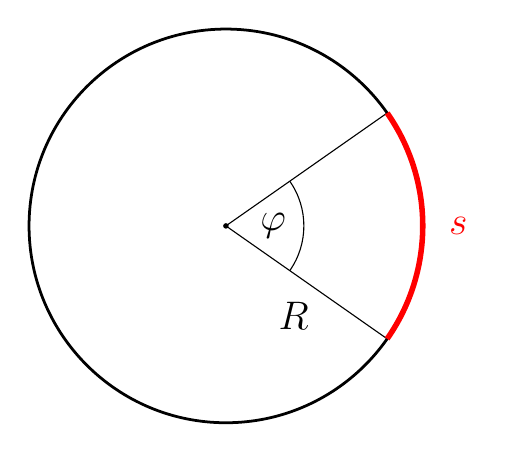
\begin{tikzpicture}
        \def\radius{2.5}
        \def\angle{35}
        % Kreis
        \draw[black, line width=1.0pt] (0,0) circle (\radius);
        \fill (0,0) circle (1.0pt);
        % Radien
        \draw (0,0) -- (-\angle:\radius) node[pos=0.42, below=7.0pt] {\Large $R$};
        \draw (0,0) -- (\angle:\radius);
        % Winkel phi
        \draw (-\angle:0.99) arc (-\angle:\angle:0.99);
        \node at (0:0.6) {\Large $\varphi$};
        % Bogen s
        \draw[red, line width=2.0pt] (-\angle:\radius) arc (-\angle:\angle:\radius);
        \node[red] at (0:\radius+0.45) {\Large $s$};
    \end{tikzpicture}
    }
    \caption{Die Bogenlänge $s$ (rote Linie) eines Kreissektors mit Radius $R$ und Öffnungswinkel $\varphi$.}\label{fig: bogenlaenge}
\end{figure}
\subsubsection{Winkelgeschwindigkeit $\omega$}
Der (zeitlich veränderliche) Betrag der Geschwindigkeit ist weiterhin definiert als das Verhältnis von zurückgelegtem Weg und verstrichener Zeit. Damit ergibt sich für die Kreisbewegung, bei der der zurückgelegte Weg gleich der Bogenlänge $s$ ist, dass 
\begin{equation}\label{eq: betrag_geschwindigkeit_kreisbewegung}
    |\ivec{v}(t)| = v(t) = \frac{\dd s}{\dd t} = \underbrace{\frac{\dd s}{\dd \varphi}}_{= R} \cdot \underbrace{\frac{\dd \varphi}{\dd t}}_{\eqdef \omega} = R\cdot \omega \mDot
\end{equation}
Da die Abhängigkeit der Bogenlänge $s$ von der Zeit $t$ zunächst nicht direkt bekannt ist, haben wir die Ableitung $\dd s/\dd t$ mittels Kettenregel in zwei Anteile zerlegt. Der erste Anteil, $\dd s/\dd \varphi$ lässt sich einfach aus der Definition der Bogenlänge bestimmen, denn für $s = R\cdot \varphi \implies \dd s/\dd \varphi = R$. Der zweite Anteil ($\dd \varphi/\dd t$) -- die Änderung des Winkels mit der Zeit -- ist die sogenannte Winkelgeschwindigkeit $\omega$. 
\begin{importantbox}[]{Definition Winkelgeschwindigkeit}
Die Winkelgeschwindigkeit $\omega$ ist definiert als 
\begin{equation}\label{eq: def_winkelgeschwindigkeit_omega}
    \omega \defeq \frac{\dd \varphi}{\dd t}\mDot
\end{equation}
Sie gibt das Verhältnis aus zurückgelegtem Winkel $\dd \varphi$ und verstrichener Zeit $\dd t$ an. Die Maßeinheit der Winkelgeschwindigkeit ist $[\omega] = \SI{1}{\radian\per\second}$. 
\end{importantbox}
Die Winkelgeschwindigkeit ist demnach unabhängig vom Radius und somit eine praktikable Größe bei der Beschreibung von Kreisbewegungen. Die Definition in \cref{eq: def_winkelgeschwindigkeit_omega} kann auch umgestellt werden zu $\dd \varphi = \omega \cdot \dd t $, was für $\omega = \const$ elementar integriert wird zu 
\begin{equation}\begin{gathered}
    \int \dd \varphi = \int \omega\cdot  \dd t \\
    \varphi(t) = \omega \cdot t + \varphi_0 \mDot
\end{gathered}\end{equation}
Die Integrationskonstante ist hier der Startwinkel $\varphi_0 = \varphi(t=0)$. Äquivalent zum Zusammenhang zwischen Ort, Zeit und Geschwindigkeit, $s = s_0 +  v\cdot t$, hängen bei der Kreisbewegung die Größen Winkel, Zeit und Winkelgeschwindigkeit zusammen, $\varphi = \varphi_0 + \omega \cdot t$. 


\subsubsection{Geschwindigkeit}\label{subsubsec: geschwindigkeit_ebeneKreisbewegung}
Der Betrag des Geschwindigkeitsvektors ist laut \cref{eq: betrag_geschwindigkeit_kreisbewegung} $|\ivec{v}(t)| = v(t) = R \cdot \omega$. Die Richtung des Geschwindigkeitsvektors $\ivec{e}_v$ kann in Polarkoordinaten deutlich einfacher ermittelt werden. Ohne Beschränkung der Allgemeinheit betrachten wir einen Massenpunkt auf einer Kreisbahn (gegen den Uhrzeigersinn) mit Radius $R$ um den Ursprung. Für die zeitabhängigen Koordinaten gilt nun geometrisch:
\begin{equation}\label{eq: koordinaten_xy_kreisbewegung}\begin{aligned}
x(t) &= R \cdot \cos(\varphi(t)) \mComma \\
y(t) &= R \cdot \sin(\varphi(t)) \mDot
\end{aligned}\end{equation}
\begin{figure}[tbh]
    \centering
    \resizebox{0.5\linewidth}{!}{
    \begin{tikzpicture}[
        scale=2,
        axis/.style={->, >=Latex, line width=1.5pt}
    ]
    \definecolor{darkerRed}{RGB}{222, 40, 73}
    \def\axislength{3.0cm}    % The radius of the circle
    \def\radius{2.5cm}    % The radius of the circle
    \def\angleEnd{55}    % The angle phi in degrees
    % Draw the x-axis
    \draw[axis] (-\axislength,0) -- (\axislength,0) node[anchor=north west] {\LARGE $x$};
    \draw[axis] (0,-\axislength) -- (0,\axislength) node[anchor=south east] {\LARGE $y$};
    % --- Draw the circular path and sector ---
    \draw[line width=0.8pt] (0,0) circle (\radius);
    \fill[red!15, draw=black] (0,0) -- (\radius,0) arc (0:\angleEnd:\radius) -- cycle;
    % --- Add labels and annotations ---
    \draw[-, >=Latex] (0.8,0) arc (0:\angleEnd:0.8cm);
    \node at (\angleEnd/2:0.54cm) {\Large $\varphi (t)$};
    \node at (-\radius/2, 0.25) {\LARGE $R$};

    \coordinate (p) at (\angleEnd:\radius); % Define the point on the circle
    \coordinate (px) at (1.434,0); % px = r * cos(phi) = 2.5*cos(55°) = 1.434
    \draw[red, line width=1.8pt, ->, >=Latex] (\radius,0) arc (0:\angleEnd/2:\radius);
    \draw[red, line width=2.0pt] (\radius,0) arc (0:\angleEnd:\radius);
    % red vectors
    \draw[->, >={Latex[length=6mm]}, darkerRed, line width=2.0pt] (0,0) -- (p) node[left=2pt, pos=0.7] {\LARGE $\ivec{r}(t)$};
    \draw[line width=1.6pt, dashed, darkerRed] (px) -- (p) node[midway, right=3pt] {\Large $y(t)$};
    \draw[line width=1.6pt, dashed, darkerRed] (0,0.01) -- (1.434,0.01) node[midway, below=3pt] {\Large $x(t)$};
    \node[circle, fill=black, inner sep=1.9pt] at (p) {};
    \end{tikzpicture}
    }
    \caption{Bei der ebenen Kreisbewegung zeigt der Ortsvektor $\protect\ivec{r}(t)$ vom Ursprung zur Position am Kreis. Die $x$- und $y$-Koordinaten können durch den Kosinus und Sinus des Winkels $\varphi(t)$ angegeben werden.}\label{fig: kreisbewegung_v_tangential}
\end{figure}
Setzen wir $\varphi(t) = \omega \cdot t + \varphi_0$ in \cref{eq: koordinaten_xy_kreisbewegung} ein, erhalten wir die Bewegungsgleichungen der ebenen Kreisbewegung. 
\begin{importantbox}{Bewegungsgleichungen der ebenen Kreisbewegung}
    Die Bewegungsgleichungen eines Massenpunktes bei der ebenen, gleichförmigen Kreisbewegung mit konstanter Winkelgeschwindigkeit $\omega$ ($\omega = \const$) um den Ursprung $M=\ipTwo{0}{0}$ sind: 
    \begin{equation}\label{eq: kreisbewegung_xy_polarkoord}\begin{aligned}
        x(t) &= R \cdot \cos(\omega t + \varphi_0)  \\
        y(t) &= R \cdot \sin(\omega t + \varphi_0)
    \end{aligned}\end{equation}
    Der Ortsvektor des Massenpunktes ergibt sich damit allgemein zu: 
    \begin{equation}\label{eq: ortsvektor_gleichf_kreisbewegung_polar}
        \ivec{r}(t) = R \icolTwo{\cos(\omega t + \varphi_0)}{\sin(\omega t + \varphi_0)} = R \cdot \ivecS{e}{r}(t)\mDot
    \end{equation} 
\end{importantbox}
Der radiale Einheitsvektor $\ivecS{e}{r}(t)$ zeigt immer vom Ursprung des Kreises zur Position des Massenpunktes am Kreis. Ist der Mittelpunkt der Kreisbewegung nicht der Ursprung, dann muss zu \cref{eq: ortsvektor_gleichf_kreisbewegung_polar} noch der Ortsvektor des Ursprungs ($\ivecS{r}{M} = \inlrowTwo{x_M}{y_M}^\T$) addiert werden: 
\begin{equation}
    \ivec{r}(t) = \ivecS{r}{M} + R\cdot \ivecS{e}{r}(t) = \icolTwo{x_M}{y_M} + R \icolTwo{\cos(\omega t + \varphi_0)}{\sin(\omega t + \varphi_0)} \mDot
\end{equation}
Nun berechnen wir den zeitabhängigen Geschwindigkeitsvektor über die Ableitung des Ortsvektors aus \cref{eq: ortsvektor_gleichf_kreisbewegung_polar}, wobei wir \oBdA $\varphi_0 = 0$ und $\ivecS{r}{M} = \ivec{0}$ setzen: 
\begin{equation}\label{eq: herleitung_geschwvektor_gleichf_kreisbew}
     \ivec{v}(t) = \frac{\dd \ivec{r}(t)}{\dd t} = \frac{\dd}{\dd t} \bigg[ R \underbrace{\icolTwo{\cos(\omega t)}{\sin(\omega t) }}_{\ivecS{e}{r}} \bigg] = R \cdot \omega \underbrace{\icolTwo{-\sin(\omega t)}{\cos(\omega t)}}_{\ivecS{e}{v}} \mDot
\end{equation}
\begin{figure}[tb]
    \centering
    \resizebox{0.50\linewidth}{!}{
    \begin{tikzpicture}[
            scale=2,
            axis/.style={->, >=Latex, line width=1.8pt},
        ]
        \def\radius{2cm}    % The radius of the circle
        \def\vlength{1.2cm}
        \def\angleEnd{40}    % The angle phi in degrees
        \definecolor{darkerRed}{RGB}{222, 40, 73}
        % Draw the x,y-axis
        \draw[axis] (-2.5,0) -- (2.5,0) node[anchor=north west] {\LARGE $x$};
        \draw[axis] (0,-2.5) -- (0,2.5) node[anchor=south east] {\LARGE $y$};
        % Draw the main circle outline
        \draw[line width=0.8pt] (0,0) circle (\radius);        
        % --- Add labels and annotations ---
        \draw[->, >=Latex] (0.7,0) arc (0:\angleEnd:0.7cm);
        \node at (\angleEnd/2:0.44cm) {\LARGE $\varphi$};
        \coordinate (p) at (\angleEnd:\radius); % Define the point on the circle | (1.53209, 1.28558)
        \coordinate (px) at (1.532,0); % Define the point on the circle
        % blue vector
        \draw[->, >={Latex[length=5mm]}, blue, line width=2.0pt] (p) -- ++(\angleEnd+90:\vlength) node[above=8.0pt, pos=0.2] {\Large $\ivec{v}(t)$};
        \draw[line width=1.9pt, dashed, blue] (p) -- (0.760744, 1.28558) node[pos=0.7, below=3pt] {\Large $v_x$};
        \draw[line width=1.9pt, dashed, blue] (0.760744, 1.28558) -- (0.760744, 2.20483) node[pos=0.4, left=3pt] {\Large $v_y$};
        % red vectors
        \draw[->, >={Latex[length=5mm]}, darkerRed, line width=2.0pt] (0,0) -- (p) node[left=6pt, pos=0.6] {\Large $\ivec{r}(t)$};
        \draw[line width=1.9pt, dashed, darkerRed] (px) -- (p) node[midway, right=3pt] {\Large $y$};
        \draw[line width=1.9pt, dashed, darkerRed] (0,0.012) -- (1.532,0.012) node[midway, below=3pt] {\Large $x$};
        \node[circle, fill=blue, inner sep=1.5pt] at (p) {};
        \end{tikzpicture}
        }
    \caption{Ein Geschwindigkeitsvektor $\protect\ivec{v}(t)$ (blauer Pfeil) steht immer senkrecht auf den Ortsvektor $\protect\ivec{r}(t)$ (roter Pfeil).}\label{fig: geschw_senkrecht_ortsvektor_kreisbew}
\end{figure}
\begin{importantbox}{Geschwindigkeitsvektor $\ivec{v}(t)$ der gleichförmigen Kreisbewegung}
    Der Geschwindigkeitsvektor der gleichförmigen ebenen Kreisbewegung lautet ganz allgemein
    \begin{equation}\label{eq: geschwindigkeit_gleichf_kreisbew}
        \ivec{v}(t) = v \cdot \ivecS{e}{v} = (R \cdot \omega) \icolTwo{-\sin(\omega t + \varphi_0)}{\cos(\omega t + \varphi_0)}
    \end{equation}
    und steht immer senkrecht auf den Ortsvektor $\ivec{r}(t)$. Die Geschwindigkeit zeigt damit in Richtung der Tangente an die Kreisbahn (siehe \cref{fig: geschw_senkrecht_ortsvektor_kreisbew}). Der Betrag der Geschwindigkeit  
    \begin{equation}\label{eq: betrag_geschwindigkeit_gleichf_kreisbew}
        v = R \cdot \omega
    \end{equation}
    ist unabhängig von der Zeit. Die Einheit der Geschwindigkeit ist weiterhin $[v] = [R \cdot \omega] = \si{\meter\per\second}$. 
\end{importantbox}
Wir können mithilfe des Skalarproduktes zeigen, dass der Einheitsvektor der Geschwindigkeit $\ivecS{e}{v}$ senkrecht auf den Einheitsvektor des Ortes $\ivecS{e}{r}$ steht:
\begin{gather*}
    \ivecS{e}{v} \cdot \ivecS{e}{r} = \icolTwo{-\sin(\omega t)}{\cos(\omega t)} \cdot \icolTwo{\cos(\omega t)}{\sin(\omega t)} = -\sin(\omega t)\cos(\omega t) + \cos(\omega t)\sin(\omega t) = 0 \\
    \implies  \ivecS{e}{v} \perp \ivecS{e}{r} \mDot
\end{gather*}
Das kann auch geometrisch anhand von \cref{fig: geschw_senkrecht_ortsvektor_kreisbew} leicht überprüft werden. Für den Ortsvektor gilt, dass $\frac{y}{x} = \tan(\varphi)$ ist, während für den Geschwindigkeitsvektor $\frac{v_y}{v_x} = -\tan^{-1}(\varphi) = \tan(\varphi + \pi/2)$. Die letzte Gleichheit ist ein bekanntes Theorem für den Tangens. Sei die Richtung des Ortsvektors durch $\varphi$ gegeben, so ist die Richtung des Geschwindigkeitsvektors demnach $\varphi + \pi/2$ (bei mathematisch positiver Umlaufrichtung).  


\subsubsection{Beschleunigung}\label{subsubsec: beschleunigung_gleichf_kreisbew}
Die Beschleunigung der gleichförmigen Kreisbewegung kann ebenso geometrisch und analytisch berechnet werden. Zunächst betrachten wir die geometrische Herleitung des Betrags der Beschleunigung 
\begin{equation}
    a(t) = |\ivec{a}(t)| =  \lim_{\Delta t \to 0} \left|\frac{\Delta \ivec{v}(t)}{\Delta t} \right| = \left| \frac{\dd \ivec{v}(t)}{\dd t} \right| \mComma
\end{equation}
wobei hier $\Delta \ivec{v}(t) = \ivec{v}(t+\Delta t) - \ivec{v}(t)$.
\paragraph{Geometrische Betrachtung}
Man betrachte eine gleichförmige Kreisbewegung mit Radius $R$ und Mittelpunkt $C$ zu zwei verschiedenen Zeitpunkten mit Positionen $A$ und $B$, dargestellt in \cref{fig: beschleunigung_geometrisch_aehnliche_dreiecke}. Das Dreieck $\triangle ABC$ ist ein gleichschenkeliges Dreieck mit Seitenlänge $R$. Der spitze Winkel $\Delta \varphi$ hat eine gegenüberliegende Seitenlänge $\Delta \ivec{r} = \ivecS{r}{B}-\ivecS{r}{A}$ (blaue, strichlierte Linie). Da die Geschwindigkeitsvektoren $\ivecS{v}{A}$ und $\ivecS{v}{B}$ senkrecht auf ihre Ortsvektoren stehen und ihre Beträge gleich sind ($|\ivecS{v}{A}| = |\ivecS{v}{B}| = v$), ist das Dreieck, das von $\ivecS{v}{A}$, $\ivecS{v}{B}$ und $\Delta\ivec{v}$ gebildet wird, ein ähnliches Dreieck zum Dreieck $\triangle ABC$.
\begin{figure}[tb]
    \centering
    \resizebox{0.65\linewidth}{!}{
    \begin{tikzpicture}[
        vec/.style={-{Stealth}, ultra thick, green!50!black},
        point/.style={fill, circle, inner sep=1.pt}
        ]
        \def\myradius{4.5cm} % Radius des Kreises
        \def\angleA{110}     % Winkel für Punkt A (in Grad)
        \def\angleB{140}     % Winkel für Punkt B (in Grad)
        \def\vecLen{3cm}      % Länge der Geschwindigkeitsvektoren
        \def\fontSize{\large}
        % --- 2. Koordinaten definieren ---
        \coordinate (C) at (0,0);
        \coordinate (A) at (\angleA:\myradius);
        \coordinate (B) at (\angleB:\myradius);
        \coordinate (M_chord) at ($(A)!0.35!(B)$);
        \coordinate (M_arc) at ({(5*\angleA+5*\angleB)/(10)}:\myradius);
        % --- 3. Kreisbahn zeichnen ---
        \draw[thick] (\angleA-20:\myradius) arc (\angleA-20:\angleB+25:\myradius);    
        \draw[line width=2.2pt,red] (\angleA:\myradius) arc (\angleA:\angleB:\myradius);    
        % --- 4. Radien und Punkte zeichnen ---
        \draw (C) -- (A) node[pos=0.5, right=2pt] {\fontSize $R$};
        \draw (C) -- (B) node[pos=0.5, below left=1pt] {\fontSize $R$};
        % --- 5. Winkel und Bogenlänge beschriften ---
        \draw[-{Stealth}] (\angleA:1.8cm) arc (\angleA:\angleB:1.8cm);
        \node at ({(\angleA+\angleB)/2}:1.3cm) {\fontSize $\Delta \varphi$};
        % --- 6. Geschwindigkeitsvektoren ---
        \draw[vec] (A) -- ++(\angleA+90:\vecLen) node[pos=0.5, above=3.0pt] {\fontSize $\ivecS{v}{A}$};
        \draw[vec] (B) -- ++(\angleB+90:\vecLen) node[pos=0.5, above left=0.2pt] {\fontSize $\ivecS{v}{B}$};
        \draw[dashed, blue, line width=1.1pt] (A) -- (B);
        % Für Δr: Linie vom Mittelpunkt der Sehne (A)--(B)
        \draw[-, thick, blue] (M_chord) -- (-1.7,2.6) node[below] {\fontSize $\Delta \ivec{r}$};
        % Für Δs: Linie vom Mittelpunkt des Bogens zwischen A und B
        \draw[-, thick,red] (M_arc) -- (-2.3,3.1) node[below=0.0pt] {\fontSize $\Delta s$};
        \node[point, label={[label distance=3pt]below:C}] at (C) {};
        \node[point, label={[label distance=0pt]above:A}] at (A) {};
        \node[point, label={[label distance=2pt]below:B}] at (B) {};
    
        % zweiter Teil: 
        \coordinate (F) at (-1.8*\myradius,0.7*\myradius);
        \coordinate (TipV1) at ($(F) + (\angleA+90:\vecLen)$);
        \coordinate (TipV2) at ($(F) + (\angleB+90:\vecLen)$);
        \draw[vec] (F) -- (TipV1) node[pos=0.5, above=3.0pt] {\fontSize $\ivecS{v}{A}$};
        \draw[vec] (F) -- (TipV2) node[pos=0.5, below right=0.2pt] {\fontSize $\ivecS{v}{B}$};
        \draw[vec] (TipV1) -- (TipV2) node[pos=0.5, left=4.5pt] {\fontSize $\Delta \ivec{v}$};
        \draw[-{Stealth}] (F)++(\angleA+90:1.1) arc (\angleA+90:\angleB+90:1.1cm);
        \draw[-, thick]  ($(F)-(0.6,0.4)$) -- +(0.2,0.6) node[above=0.0pt] {\fontSize $\Delta \varphi$};
    \end{tikzpicture}
    }
    \caption{Geometrische Herleitung der Beschleunigung. Die Dreiecke $(ABC)$ und ($\protect\ivecS{v}{1}, \protect\ivecS{v}{2}, \Delta\protect\ivec{v}$) sind ähnlich, da beide gleichschenklige Dreiecke mit dem selben spitzen Winkel sind.}\label{fig: beschleunigung_geometrisch_aehnliche_dreiecke}
\end{figure}
Daraus erhalten wir die Beziehung:
\begin{equation}\label{eq: verhältnis_dv_dr_gleichf_kreisbew}
    \frac{|\Delta \ivec{r}|}{R} = \frac{|\Delta \ivec{v}|}{v} \implies |\Delta \ivec{v}| = \frac{v}{R} |\Delta \ivec{r}| \mDot
\end{equation}
Nun dividieren wir \cref{eq: verhältnis_dv_dr_gleichf_kreisbew} durch $|\Delta t|$ und bilden den Limes $\Delta t\to 0$, bei dem die endlichen Differenzen in Differentiale übergehen, und erhalten somit einen Ausdruck für den Betrag der Beschleunigung
\begin{equation}\label{eq: betrag_beschl_gleichf_kreisbew_noch_mit_limes}
    \lim_{\Delta t\to 0}\left|\frac{\Delta \ivec{v}}{\Delta t}\right| = \left| \frac{\dd \ivec{v}}{\dd t} \right| = |\ivec{a}(t)| = \lim_{\Delta t\to 0} \frac{v}{R} \left|\frac{\Delta \ivec{r}}{\Delta t}\right| \mDot
\end{equation}
\Cref{eq: betrag_beschl_gleichf_kreisbew_noch_mit_limes} enthält auf der rechten Seite allerdings noch den Ausdruck $|\Delta \ivec{r}/\Delta t|$, der die Sehnenlänge $|\Delta \ivec{r}|$ enthält. Für endliche Winkeländerungen $\Delta \varphi$ entspricht die Sehnenlänge nicht dem zurückgelegten Weg des Massenpunktes (siehe \cref{fig: beschleunigung_geometrisch_aehnliche_dreiecke}), weshalb $|\Delta \ivec{r}/\Delta t| \neq |\ivec{v}(t)|$ ist. In \cref{subsec: herleitung_bogenlaenge_sehnenlaenge} haben wir jedoch gezeigt, dass
\begin{equation}
    \lim_{\Delta t \to 0} |\Delta \ivec{r}| = \Delta s
\end{equation} 
[siehe \cref{eq: sehnenlänge_gleich_bogenlänge}] -- \gDh die Länge der Sehne $\overline{AB}$ konvergiert im Grenzübergang $\Delta t \to 0$ gegen die Bogenlänge. \\

Schließlich können wir im Limes die Sehnenlänge durch die Bogenlänge ersetzen und somit wird $\lim_{\Delta t \to 0} |\Delta \ivec{r}/\Delta t| = v$. In \cref{eq: betrag_beschl_gleichf_kreisbew_noch_mit_limes} wird der Betrag der Beschleunigung dann
\begin{equation}
    a(t) = |\ivec{a}(t)| = \lim_{\Delta t \to 0} \frac{v}{R} \left| \frac{\Delta \ivec{r}}{\Delta t} \right|  = \frac{v}{R} \cdot v = \frac{v^2}{R}
\end{equation}
Um die Richtung des Beschleunigungsvektors zu bestimmen, verwenden wir zunächst die Tatsache, dass der Geschwindigkeitsvektor $\ivec{v}(t)$ normal auf den Ortsvektor $\ivec{r}(t)$ steht und parallel zum differentiellen Verschiebungsvektor\footnote{Die geschlossene Formel für den differentiellen Verschiebungsvektor lautet \begin{equation}
    \dd \ivec{r} =  \left[\lim_{\Delta t \to 0} \left(\frac{\ivecS{r}{B} - \ivecS{r}{A}}{\Delta t}\right)\right] \dd t = \ivec{v} \dd t \mDot
\end{equation}} $\dd \ivec{r}$ ist: 
\begin{equation}\label{eq: er_perp_ev_parallel_dr}
    \ivecS{e}{r} \perp \ivecS{e}{v} \quad\mAND\quad \ivecS{e}{v} \parallel \dd \ivec{r} \mDot
\end{equation}
Dann muss aber der differentielle Geschwindigkeitsvektor\footnote{Die geschlossene Formel für den differentiellen Geschwindigkeitsvektor lautet \begin{equation}
    \dd \ivec{v} =  \left[\lim_{\Delta t \to 0} \left(\frac{\ivecS{v}{B} - \ivecS{v}{A}}{\Delta t}\right)\right] \dd t = \ivec{a} \dd t \mDot
\end{equation}}, $\dd \ivec{v}$,
\begin{equation}
    \dd \ivec{v} \parallel \ivecS{e}{a} \quad\mAND\quad \ivecS{e}{a} \perp \ivecS{e}{v}
\end{equation}
sein. Dass $\dd \ivec{v} \parallel \ivecS{e}{a}$, erschließt sich aus der Definition der Beschleunigung, $\ivec{a} = \dd \ivec{v}/\dd t$. Die Orthogonalität von $\ivecS{e}{a}$ mit $\ivecS{e}{v}$ ist bedingt durch $\ivec{r} \perp \ivec{v}$ und daher $\ivec{v} \perp \ivec{a}$. Es gilt daher, dass 
\begin{equation}
    \ivecS{e}{a} = -\ivecS{e}{r} 
\end{equation}
ist und somit zeigt der Beschleunigungsvektor $\ivec{a}$ zum Mittelpunkt des Kreises (antiparallel zum Ortsvektor) 
\begin{equation}
    \ivec{a}(t) = \frac{v}{R^2} \ivecS{e}{a} = -\frac{v}{R^2} \ivecS{e}{r}\mDot
\end{equation}



\paragraph{Analytische Betrachtung}
Die analytische Betrachtung geht von der Definition der Beschleunigung aus und führt die Differentiation mithilfe der Produktregel (siehe \cref{sec: Ableitungsregeln}) aus:
\begin{equation}
    \ivec{a}(t) = \frac{\dd \ivec{v}(t)}{\dd t} = \frac{\dd}{\dd t}(v \cdot \ivecS{e}{v}) = \underbrace{\frac{\dd v}{\dd t}}_{=0} \cdot \ivecS{e}{v} + v \cdot \frac{\dd \ivecS{e}{v}}{\dd t} = v \cdot \frac{\dd \ivecS{e}{v}}{\dd t} \mDot
\end{equation}
Die Änderung des Betrages der Geschwindigkeit verschwindet ($\dd v/\dd t = 0$), weil bei der gleichförmigen Kreisbewegung $v = \const$. 
Die Ableitung des Einheitsvektors $\ivecS{e}{v}$ der Geschwindigkeit (siehe \cref{eq: geschwindigkeit_gleichf_kreisbew}) ist
\begin{equation}
    \frac{\dd \ivecS{e}{v}}{\dd t} = \frac{\dd}{\dd t} \icolTwo{-\sin(\omega t)}{\cos(\omega t)} = -\omega \underbrace{\icolTwo{\cos(\omega t)}{\sin(\omega t)}}_{= \ivecS{e}{r}}  = -\omega \cdot \ivecS{e}{r} \mComma
\end{equation}
wobei wir wieder \oBdA $\varphi_0 = 0$ gewählt haben. Damit erhält man für den Beschleunigungsvektor
\begin{equation}
    \ivec{a}(t) = v \cdot \frac{\dd \ivecS{e}{v}}{\dd t} = v \cdot (-\omega \cdot \ivecS{e}{r}) = -(v \cdot \omega) \cdot \ivecS{e}{r} = - \frac{v^2}{R} \ivecS{e}{r}\mDot
\end{equation}
\begin{importantbox}{Zentripetalbeschleunigung $\ivec{a}(t)$}
    Der Beschleunigungsvektor der ebenen Kreisbewegung lautet
    $$ \ivec{a}(t) = a \cdot \ivecS{e}{a} = -\frac{v^2}{r} \cdot \ivecS{e}{r} = -\omega^2 \cdot r \cdot \ivecS{e}{r} $$
    und zeigt zum Kreismittelpunkt. Deshalb nennt man sie Zentripetalbeschleunigung (\gDQ{mittelpunktsuchende Beschleunigung}). Ihre Einheit beträgt $[\frac{v^2}{r}] = \si{\meter\per\second\squared}$.
\end{importantbox}

\section{Die allgemeine krummlinige Bewegung}
Bei der gleichförmigen Kreisbewegung nimmt die Beschleunigung eine sehr einfache Form an, da der Betrag der Geschwindigkeit konstant ist, $|\ivec{v}| = \const$. Im allgemeinen Fall wird sich $\ivec{v}$ aber nach Betrag und Richtung ändern und zwar weil sich die Beschleunigung sowohl nach Betrag als auch nach Richtung ändert. \\

Die Geschwindigkeit $\ivec{v}$ steht jedoch -- unabhängig von der Bewegungsform -- immer tangential zur Bahnkurve. Es ergibt sich nämlich aus der Definition $\ivec{v} = \frac{\dd \ivec{r}}{\dd t}$, dass die Geschwindigkeit parallel zur differentiellen Verschiebung ist. Die Beschleunigung $\ivec{a}$ kann eine beliebige Richtung aufweisen und lässt sich in zwei Komponenten zerlegen: 

\begin{importantbox}{Beschleunigung bei der krummlinigen Bewegung}
Die Beschleunigung $\ivec{a}(t)$ kann im Allgemeinen eine beliebige Richtung aufweisen
    \begin{equation}
        \ivec{a}(t) = \frac{\dd \ivec{v}(t)}{\dd t} = \frac{\dd}{\dd t}(v(t) \cdot \ivecS{e}{v}(t)) = \underbrace{\frac{\dd v(t)}{\dd t} \cdot \ivecS{e}{v}(t)}_{\ivecS{a}{t}(t)} + \underbrace{v(t) \cdot \frac{\dd \ivecS{e}{v}(t)}{\dd t}}_{\ivecS{a}{n}(t)} = \ivecS{a}{t}(t) + \ivecS{a}{n}(t)
    \end{equation}
und in die Tangential- und Normalbeschleunigung zerlegt werden.
\end{importantbox}
\begin{figure}
    \centering
    \includegraphics[width=0.65\linewidth]{Bilder/Kapitel_Mechanik/Kapitel_Kinematik/krummlinigeBewBahnkurve.png}
    \caption{Die Geschwindigkeit $\protect\ivec{v}(t)$ steht immer tangential auf die Bahnkurve. Die Beschleunigung hat jedoch zwei Anteile, die normal aufeinander stehen: die Tangentialbeschleunigung $\protect\ivecS{a}{t}$ und die Normalbeschleunigung $\protect\ivecS{a}{n}$.}\label{fig: allg_krummlinige_bewegung}
\end{figure}
\begin{rememberbox}{Tangential- und Normalbeschleunigung}
    \begin{itemize}
        \item \textbf{Die Tangentialbeschleunigung $\ivecS{a}{t} = \frac{\dd v}{\dd t} \cdot \ivecS{e}{v}$} ist ein Vektor, der in Tangentialrichtung der Bahnkurve zeigt, also parallel zu $\ivec{v}$. Sein Betrag $|\ivecS{a}{t}| = \frac{\dd v}{\dd t}$ beschreibt die Änderungsrate des Betrages der Geschwindigkeit.
        \item \textbf{Die Normalbeschleunigung $\ivecS{a}{n} = v \cdot \frac{\dd\ivecS{e}{v}}{\dd t}$} ist ein Vektor, der senkrecht auf die Geschwindigkeit und damit senkrecht auf die Tangente steht. Dieser Anteil beschreibt die Änderung der Richtung der Geschwindigkeit.
    \end{itemize}
\end{rememberbox}
Während die Tangentialbeschleunigung also die umgangssprachliche Erhöhung (bzw. Verringerung) der Geschwindigkeit bewirkt, veranlasst die Normalbeschleunigung einen Richtungswechsel und lenkt den Massenpunkt sozusagen. 

% Chapter end - always start new page after chapter
\newpage